\documentclass[main.tex,fontsize=8pt,paper=a4,paper=landscape,DIV=calc,]{scrartcl}
% Document
\usepackage[T1]{fontenc}
\usepackage[dvipsnames]{xcolor}
\usepackage[nswissgerman,english]{babel}
\renewcommand{\familydefault}{\sfdefault}

% Format
\usepackage[top=5mm,bottom=1mm,left=5mm,right=5mm]{geometry}
%\setlength{\headheight}{\baselineskip}
%\setlength{\headsep}{0mm}

%\usepackage{scrlayer-scrpage}
%\clearpairofpagestyles
%\chead{{\bfseries\TITLE, \AUTHOR, \pagename~\thepage}}

%\addtokomafont{pagehead}{\upshape}

\usepackage{multicol}
\setlength{\columnsep}{2mm}
\setlength{\columnseprule}{0.1pt}

% Math
\usepackage{amsmath}
\usepackage{amssymb}
\usepackage{amsfonts}

% Code
\usepackage{fancyvrb, etoolbox, listings, xcolor}
%\usemintedstyle{bw}

%\newminted[shell]{bash}{
%fontsize=\footnotesize,
%fontfamily=tt,
%breaklines=true,
%frame=single,
%framerule=0.1pt,
%framesep=2mm,
%tabsize=2
%}
%\newminted{css}{
%breaklines=true,
%tabsize=4,
%autogobble=true,
%escapeinside=||,
%stripall=true,
%stripnl=true,
%}

    \definecolor{lightgray}{rgb}{0.95, 0.95, 0.95}
    \definecolor{darkgray}{rgb}{0.4, 0.4, 0.4}
    \definecolor{purple}{rgb}{0.65, 0.12, 0.82}
    \definecolor{ocherCode}{rgb}{1, 0.5, 0} % #FF7F00 -> rgb(239, 169, 0)
    \definecolor{blueCode}{rgb}{0, 0, 0.93} % #0000EE -> rgb(0, 0, 238)
    \definecolor{greenCode}{rgb}{0, 0.6, 0} % #009900 -> rgb(0, 153, 0)
    \definecolor{teal}{rgb}{0.0, 0.5, 0.5}

\lstdefinestyle{code}{
    identifierstyle=\color{black},
    keywordstyle=\color{blue}\bfseries\small,
    ndkeywordstyle=\color{greenCode}\bfseries\small,
    stringstyle=\color{ocherCode}\ttfamily\small,
    commentstyle=\color{teal}\ttfamily\textit\small,
    basicstyle=\ttfamily\small,
    breakatwhitespace=false,         
    breaklines=true,                 
    captionpos=b,                    
    keepspaces=true,                 
    showspaces=false,                
    showstringspaces=false,
    showtabs=false,                  
    tabsize=2,
    belowskip=-5pt
}



% Images
\usepackage{graphicx}
\newcommand{\pic}{\includegraphics[scale=0.3]}
\graphicspath{{Screenshots/}{../Screenshots}}
\makeatletter
\def\pictext#1#2{%
    \@ifnextchar[{%
    \pictext@iiiii{#1}{#2}%
    }{%
      \pictext@iiiii{#1}{#2}[0.5,0.4,0.3]% Default is 5
    }%
}
\def\pictext@iiiii#1#2[#3,#4,#5]{\begin{minipage}{#3\textwidth}\includegraphics[scale=#4]{#1}\end{minipage}\begin{minipage}{#5\textwidth}#2\end{minipage}}
\def\minipg#1#2{%
    \@ifnextchar[{%
    \minipg@iiii{#1}{#2}%
    }{%
      \minipg@iiii{#1}{#2}[0.3,0.6]% Default is 5
    }%
}
\def\minipg@iiii#1#2[#3,#4]{\vspace{0.8mm}\begin{minipage}{#3\textwidth}#1\end{minipage}\begin{minipage}{#4\textwidth}#2\end{minipage}{\vspace{0.8mm}}}
\makeatother

%\newenvironment{minty}[2]% environment name
%{% begin code
%  \begin{minipage}{#1}
%  \begin{minted}{#2}
%}%
%{% end code
%  \end{minted}
%  \end{minipage}
%  \end{minty}\ignorespacesafterend
%} 

% Smaller Lists
\usepackage{enumitem}
\setlist[itemize,enumerate]{leftmargin=3mm, labelindent=0mm, labelwidth=1mm, labelsep=1mm, nosep}
\setlist[description]{leftmargin=0mm, nosep}
\setlength{\parindent}{0cm}

% Smaller Titles
\usepackage[explicit]{titlesec}

%% Color Boxes
\newcommand{\sectioncolor}[1]{\colorbox{black!60}{\parbox{0.989\linewidth}{\color{white}#1}}}
\newcommand{\subsectioncolor}[1]{\colorbox{black!50}{\parbox{0.989\linewidth}{\color{white}#1}}}
\newcommand{\subsubsectioncolor}[1]{\colorbox{black!40}{\parbox{0.989\linewidth}{\color{white}#1}}}
\newcommand{\paragraphcolor}[1]{\colorbox{black!30}{\parbox{0.989\linewidth}{\color{white}#1}}}
\newcommand{\subparagraphcolor}[1]{\colorbox{black!20}{\parbox{0.989\linewidth}{\color{white}#1}}}

%% Title Format
\titleformat{\section}{\vspace{0.5mm}\bfseries}{}{0mm}{\sectioncolor{\thesection~#1}}[{\vspace{0.5mm}}]
\titleformat{\subsection}{\vspace{0.5mm}\bfseries}{}{0mm}{\subsectioncolor{\thesubsection~#1}}[{\vspace{0.5mm}}]
\titleformat{\subsubsection}{\vspace{0.5mm}\bfseries}{}{0mm}{\subsubsectioncolor{\thesubsubsection~#1}}[{\vspace{0.5mm}}]
\titleformat{\paragraph}{\vspace{0.5mm}\bfseries}{}{0mm}{\paragraphcolor{\theparagraph~#1}}[{\vspace{0.5mm}}]
\titleformat{\subparagraph}{\vspace{0.5mm}\bfseries}{}{0mm}{\subparagraphcolor{\thesubparagraph~#1}}[{\vspace{0.5mm}}]

%% Title Spacing
\titlespacing{\section}{0mm}{0mm}{0mm}
\titlespacing{\subsection}{0mm}{0mm}{0mm}
\titlespacing{\subsubsection}{0mm}{0mm}{0mm}
\titlespacing{\paragraph}{0mm}{0mm}{0mm}
\titlespacing{\subparagraph}{0mm}{0mm}{0mm}

%% format cells
\usepackage[document]{ragged2e}
\usepackage{array, makecell}
\renewcommand{\arraystretch}{2}
\newcommand{\mc}{\makecell[{{m{1\linewidth}}}]}



\renewcommand{\sectioncolor}[1]{\colorbox{black!60}{\parbox{0.97\linewidth}{\color{white}#1}}}
\renewcommand{\subsectioncolor}[1]{\colorbox{black!50}{\parbox{0.97\linewidth}{\color{white}#1}}}
\renewcommand{\subsubsectioncolor}[1]{\colorbox{black!40}{\parbox{0.97\linewidth}{\color{white}#1}}}
\renewcommand{\paragraphcolor}[1]{\colorbox{black!30}{\parbox{0.97\linewidth}{\color{white}#1}}}
\renewcommand{\subparagraphcolor}[1]{\colorbox{black!20}{\parbox{0.97\linewidth}{\color{white}#1}}}

\begin{document}
\begin{multicols*}{4}

\lstset{
    language={[x86masm]Assembler},
    style=code,
}

\section{Assembly}
Assembly is a platform -> intel, arm, risc-v dependent programming language. 
It converts instructions into binary -> machine code. Most compiled language will convert to assembly code before being compiled to binary!

\subsection{Numbers in Assembly}
\begin{itemize}
\item \textcolor{black}{db 48 -> Byte 48d}
\item \textcolor{black}{db 0x35, 0h21, 049h -> Bytes 35h, 21h, 49h}
\item \textcolor{black}{db 'a' -> ASCII-Code a == 61h == db 0x61}
\item \textcolor{purple}{db == Byte -> 8 Bit}
\item \textcolor{purple}{dw == Word -> 16 Bit == db first-nr, db second-nr}
\item \textcolor{purple}{dd == Doubleword -> 32 Bit}
\item \textcolor{purple}{dq == QuadWord -> 64 Bit}
\item \textcolor{orange}{048d -> d for decimal}
\item \textcolor{orange}{048h or 0x48 -> h for hex}
\item \textcolor{orange}{10001000b or 1000\_1000b -> b/y for binary}
\end{itemize}
\subsection{Length Calculation}
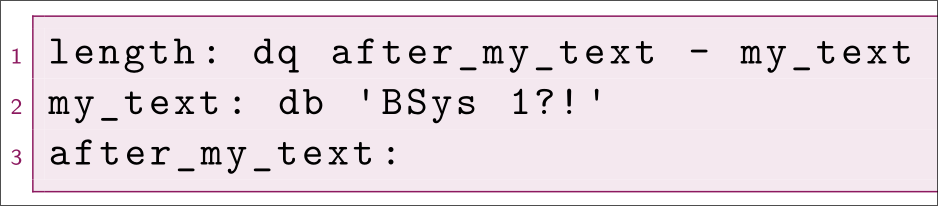
\includegraphics[scale=0.2]{2022-09-27-04:27:52.png}
first define a quadword with 2 unknown labels, then define my\_text with 'Besys',
after define aftermytext and recude the current instruction pointer with the instruction pointer at my\_text
\subsection{Default Registers}
\begin{itemize}
\item Right 8 bit register: \textcolor{purple}{AL}
\item Left 8 bit register: \textcolor{purple}{AH}
\item 16 bit register: \textcolor{purple}{AX}
\item 32 bit register: \textcolor{purple}{EAX}
\item 64 bit register: \textcolor{purple}{RAX}
\end{itemize} 

\subsection{Special Registers}
\begin{itemize}
  \item \textcolor{purple}{RAX} general use register
  \item \textcolor{purple}{RCX} Counter for loops or strings
  \item \textcolor{purple}{RDX} Pointer for I/O Operations
  \item \textcolor{purple}{RBX} Datapointer
  \item \textcolor{purple}{RSI,RDI} Source for stringoperations
  \item \textcolor{purple}{RSP} Stackpointer!!
  \item \textcolor{purple}{RBP} Basepointer
  \item \textcolor{purple}{R8-R15} additional registers
\end{itemize}
Note other registers like RBX exist as well, but aren't specifically used for something.

\subsection{Dealing with Memoryi}
Memory is accessed with the [] operators, this can also be offset with either multiplication or other calulations
\begin{lstlisting}
mov rax, [0x8000] ; ok move 8000h into rax
mov [0x8000], rax ; ok move value at rax into 0x8000
mov rax, rbx      ; ok move rbx into rax, no memory access!!
mov [0x8000], [0x7000] ; error can't move memory to memory!!
\end{lstlisting}
\vspace{2mm}

\subsection{Assembly Instructions}
\begin{itemize}
\item mov rax, 1 \textcolor{teal}{//move the value 1 into rax, keep in mind that mov can hold other operations!}
\item equ rax, 1+1 \textcolor{teal}{//arithmic operation}
\item add z,   q  \textcolor{teal}{// z + q} 
\item sub z,   q  \textcolor{teal}{// z - q}
\item adc z,   q  \textcolor{teal}{// z + q + c (carry -> previous calculation)}
\item sbb z,   q  \textcolor{teal}{// z - q - c (carry -> previous calculation)}
\item neg z       \textcolor{teal}{// 0 - z ("zweierkomplement")}
\item inc z       \textcolor{teal}{// z++ }
\item dec z       \textcolor{teal}{// z-- }
\item mul z,      \textcolor{teal}{// multiply with implicit 2.operand }\newline
mul rbx -> RDX:RAX <-- RAX * RBX
\item imul z,   i  \textcolor{teal}{// signed equivalent for mul, z * i }
\item div z,      \textcolor{teal}{// divide with implicit 2.operand}\newline
div rbx  \newline
d = RDX:RAX\newline
RAX <-- RDX:RAX / RBX\newline
RDX <-- RDX:RAX mod RBX
\item shl z,   i  \textcolor{teal}{// z * \(2^i\)               --> shift}
\item shr z,   i  \textcolor{teal}{// z * \(2^{-i}\) z signed   --> shift}
\item sar z,   i  \textcolor{teal}{// z * \(2^{-i}\) z unsigned --> shift}
\item rol z,   i  \textcolor{teal}{// Left-Rotate i Bits }
\item ror z,   i  \textcolor{teal}{// Right-Rotate i Bits }
\item and rax, rbx\textcolor{teal}{// AND}
\item not rax     \textcolor{teal}{// NOT}
\item cmp rax, 3 \textcolor{teal}{// compare rax and 3, set flag if not}
\item cmov rax, 5 \textcolor{teal}{// move 5 into rax if condition met}
\item je 230 \textcolor{teal}{// move 230 down if condition met}
\end{itemize}

\subsubsection{Flags}
\textcolor{purple}{Carry Flag (CF) == overflow with unsigned intergers}\newline
0000 + 1111 = 0000, CF = 1 --> 1 + 15 = 0, CF = 1
\textcolor{purple}{OverFlow Flag (OF) == overflow with signed integers}\newline
0011 + 0001 = 1000 -> 7 + 1 = -8 (negative prefix)
\textcolor{purple}{Zero Flag (ZF) == set when result is 0}
\textcolor{purple}{Sign Flag == is the highest bit of the result}
\textcolor{purple}{Parity Flag (PF) == set if lowest bute has an even number of bits}

\subsubsection{Usage of compare with Condition Codes}
\textcolor{teal}{A : Above } \textcolor{teal}{ -> CF = 0 AND ZF = 0}\newline
\textcolor{teal}{AE: Above or Equal } \textcolor{teal}{ -> CF = 0}\newline
\textcolor{teal}{B : Below } \textcolor{teal}{ -> CF = 1}\newline
\textcolor{teal}{BE: Below or Equal } \textcolor{teal}{ -> CF = 1 AND ZF = 1}\newline
\textcolor{teal}{E : Equal } \textcolor{teal}{ -> ZF = 1}\newline
\textcolor{teal}{G : Greater } \textcolor{teal}{ -> SF = OF = 0 AND ZF = 0}\newline
\textcolor{teal}{GE: Greater or Equal } \textcolor{teal}{ -> SF = OF}\newline
\textcolor{teal}{L : Less } \textcolor{teal}{ -> SF != OF}\newline
\textcolor{teal}{LE: Less or Equal } \textcolor{teal}{ -> SF != OF AND ZF = 1}\newline
\textcolor{teal}{PE: Parity Even}  \textcolor{teal}{ -> PF =1}\newline
\textcolor{teal}{PO: Parity Old } \textcolor{teal}{ -> PF = 0}\newline
\textcolor{teal}{Z:  Zero} \textcolor{teal}{ -> ZF = 1}

\subsection{Syscall}
Syscalls are special operations that the Operating system understands
\begin{lstlisting}
mov rax, 60 // 60 == exit instruction
mov rdi, 0 // exit code -> 0 means ok
syscall // OS executes instruction from rax
\end{lstlisting}
\vspace{2mm}



\lstset{
    language=c,
    style=code,
}

\section{C}


\section{Cache}


\section{RAM}

\end{multicols*}
\end{document}
